\chapter{Konzept zur automatisierten Schmerzbewertung anhand akustischer Signale}
\label{sec:concept}

%Ergänenzen!
In \autoref{sec:medicalFoundations} wurde die Schmerzdiagnostik mit Hilfe multimodaler Schmerz-Scales im medizinischen Alltag vorgestellt. Dieses Kapitel gibt einen Überblick über das entworfene Systemkonzept, das die Schmerzdiagnostik nach diesem Vorbild automatisiert und kontinuierlich anhand akustischer Signale vornimmt. Dazu wird in \autoref{sec:system_literature} zunächst ein Überblick über Veröffentlichungen mit ähnlichen Zielstellungen gegeben. In \autoref{sec:pipeline} werden die Verarbeitungsschritte erläutert, die von einem Eingangssignal bis zur Visualisierung der Schmerzdiagnostik führen. Da in dieser Arbeit auf der Fokus auf akustischen Signale liegt, wird in \autoref{sec:multimodal_integration} die Eingliederung des Konzeptes in ein multimodales System diskutiert.

\section{Literaturüberblick}
\label{sec:system_literature}

Ein großer Teil der Veröffentlichungen, die sich in das Feld der Analyse von Audioaufnahmen Neugeborener einordnen lassen, stellen Methoden zur Klassifizierung einzelner Schreieinheiten vor, entweder bezüglich der Weinursache (Hunger, Angst, Schmerz usw. ) oder zur Diagnose bestimmter Krankheiten. Diese Methoden sind in den meisten Fällen nicht für eine kontinuierliche Analyse vorgesehen, sondern haben das Ziel, die Eignung bestimmter Features oder Klassifizierungsalgorithmen für die jeweiligen Klassifizierung zu erforschen. Beispiele für solche Veröffentlichungen sind die von Abdulaziz et al. \cite{class_abdulaziz} oder Fuhr et al. \cite{comparisonOfLearning}.

Várallyay stellte in seiner Dissertation \glqq Analysis of the Infant Cry with Objective Methods\grqq{} \cite{cry_thesis} Methoden zur automatisierten Analyse kindlicher Lautäußerungen vor. Das primäre Ziel der Dissertation war die Erforschung der Unterschiede zwischen den Lautäußerungen gesunder und tauber Neugeborener. Die Algorithmen zur automatisierten Analyse der Audiosignale waren ein \glqq Nebenprodukt\grqq{} zur schnelleren Datenauswertung. Die Auswertung musste nicht kontinuierlich erfolgen. In der vorgestellten Verarbeitungs-Pipeline wurde das Eingangssignal in Zeitfenster weniger Millisekunden zerlegt und jedes Fenster nach Entscheidungsregeln als \emph{stimmhaft} oder \emph{nicht stimmhaft} markiert. Die stimmhaften Signalfenster wurden zu \emph{Segmenten} zusammengefasst (welche in \autoref{sec:acousticModel} als Schreieinheiten bezeichnet werden). Auf Basis der Segmente wurden Auswertungen bezüglich des Zeitbereiches (Durchschnittliche Segmentlänge, Pausenlängen, ... ), des Frequenzbereiches (Grund-Frequenz, Formanten-Frequenzen, ...) und des Melodieverlaufes vorgenommen. Analysiert wurden manuell geschnittene Audioaufnahmen von Babys mit einer Länge von 10 bis \SI{100}{\second}. Auf Basis der Auswertungsergebnisse stellte Varallyay die wichtigsten Unterscheidungsmerkmale zwischen den Lautäußerungen tauber und gesunder Babys fest. In der Dissertation \cite{cry_thesis} wird ein Überblick über das Vorgehen und die Ergebnisse gegeben. Die Verarbeitungsschritte wurden detaillierter in einzelnen Veröffentlichungen beschrieben, wobei der Autor dieser Arbeit nur den Zugriff auf einige dieser Veröffentlichungen erhalten konnte.

Cohen et al. haben 2012 in der Veröffentlichung \glqq Infant Cry Analysis and Detection\grqq{} \cite{cohenCry}  ein System zur Analyse der akustischen Signale von Neugeborenen vorgestellt. Dieses System klassifizierte die Audiosignale in eine der drei Klassen \emph{Cry, No Cry} und \emph{No Activity}. Die Klasse \emph{Cry} bezeichnet Lautäußerungen, die eine potentiell Gefahr für das Baby anzeigen, wie z.B. wie Schmerz oder Hunger. Die Klasse \emph{No Cry} bedeutete, dass das Baby zwar Laute von sich gibt, diese aber keine potentielle Gefahr signalisieren. Die Klasse \emph{No Activity} bezeichnete keinerlei Lautäußerung. Die Verarbeitungs-Pipeline wurde detailliert vorgestellt und ist für die kontinuierliche Verarbeitung mit einer gewissen Verzögerungszeit geeignet. Dabei wird ein Eingangssignal in überlappende \emph{Segmente} \`{a} \SI{10}{\second} zerlegt. Die Stimmaktivität in den Segmenten wird algorithmisch festgestellt. Wenn Aktivität vorliegt, wird das Segment in Sektionen \`{a} \SI{1}{\second} zerlegt und die Stimmaktivität für jede Sektion gemessen. Liegt eine ausreichende Stimmaktivität in einer Sektion vor, wird sie abermals in \emph{Frames} \`{a} \SI{32}{\milli\second} zerlegt und Attribute für jeden Frame errechnet. Mit Hilfe von Entscheidungsregeln werden die Frames in \emph{Cry, No-Cry} oder \emph{No Activity} klassifiziert, wobei kontextuelle Informationen der umliegenden Frames mit einbezogen werden. Aus den Klassen der Frames wird auf die Klasse der Sektion geschlossen, und aus den Klassen der Sektionen auf die Klasse des Segmentes. 

%Das System hat mit den Anforderungen dieser Arbeit gemeinsam, dass ebenfalls die kontinuierliche Verarbeitung im Vordergrund steht. Der Nachteil an dieser Methode ist, dass die zeitliche längste Einheit, für die die Klassifizierung vorgenommen wird, unflexibel auf \SI{10}{\second} festgelegt ist. Daher müsste diese Verarbeitungs-Pipeline abgewandelt werden, um anstelle der Ableitung der drei genannten Klassen einen Pain Score ableiten zu können, die einen längeren Beobachtungszeitraum als \SI{10}{\second} benötigt.

Pal et al.  haben 2006 in der Veröffentlichung \glqq Emotion detection from infant facial experessions and cries\grqq{} \cite{palEmotion} ein System vorgestellt, welches aus den akustischen Eigenschaften des Weinens die Emotion ableitet. Die zu erkennenden Emotionen waren \emph{Trauer, Wut, Hunger, Angst und Schmerz}. Es wurde nicht erwähnt, ob die Analyse kontinuierlich oder nicht kontinuierlich erfolgt. Bei der Verarbeitung der akustischen Signale wurden die Attribute \emph{Grundtonhöhe} und die \emph{Frequenz der ersten drei Formanten} extrahiert und mit einem Klassifizierungsalgorithmus klassifiziert. Es wurde nicht beschrieben, inwiefern die Eigenschaften aus kurzen Signalfenstern oder längeren Signalabschnitten errechnet wurden, welche Vorverarbeitungsschritte angewandt wurden und ob die Klassifizierung auf Ebene der Signalfenster oder über längere Zeitabschnitte hinweg geschieht.

Zamzi et al.  haben 2016 in der Veröffentlichung \glqq An Approach for Automated Multimodal Analysis of Infants' Pain\grqq{} \cite{zamziMultimodal} ein System zur automatisierten und kontinuierlichen multimodalen Analyse von Neugeborenen zur Ableitung des Schmerzes vorgestellt. Das System trägt den Namen \emph{MPAS}. Der Schmerzgrad wird aus den Analyseergebnissen der Schmerzindikatoren  \emph{Gesichtsausdruck, Körperbewegung, Vitalfunktionen} und \emph{Weinen} errechnet. Der Schmerz wird auf ein eigens entwickeltes Scoring-System abgebildet, ohne die Scoring-Systeme der Schmerzscales zu verwenden. Während in der Veröffentlichung die Analyse der genannten Schmerzindikatoren angekündigt wurde, wurden daraufhin die Methoden zur Analyse der akustischen Signale \emph{nicht} erläutert. Auch die ersten Validierungsergebnisse beziehen sich nur auf den Gesichtsausdruck, die Körperbewegung und die Vitalfunktionen. Es ist nicht klar, ob die Miteinbeziehung akustischer Signale fallen gelassen wurde. Die Ausführungen konzentrieren sich dazu vermehrt auf die Methoden zur Kombination der Auswertungsergebnisse der einzelnen Schmerzindikatoren.

H. Golub und M. Corwin erwähnten in \glqq A Physioacoustic Model of the Infant Cry\grqq{} \cite{cryModel}, bereits in den achtziger Jahren ein System zur computergestützten und voll automatisierten Analyse von Cry-Segmenten implementiert zu haben. Das System nimmt 1.) eine Audioaufnahme, gespeichert auf einer Kasette, an, 2.) berechnet Formanten, Grundfrequenz und Amplitude gegen die Zeit, 3.) samplt die Grundfrequenz-Kontur, 4.) berechnet insgesamt 88 akkumulierte Features für das gesamte Segment und 5.) zieht Schlussfolgerungen aus den 88 Eigenschaften, wie zum Beispiel die Diagnose einer bestimmten Krankheit.\cite[S. 75 - 76]{cryModel} Abseits der kurzen Erwähnung der Existenz dieses ersten automatisierten Analysesystems für das Weinen von Babys in \cite{cryModel} konnte der Autor dieser Arbeit keine Implementierungsdetails oder sonstige genauere Ausführungen über das System finden, welche für diese Arbeit von höchstem Interesse gewesen wären.


%\section{Anforderungen an das Konzept}
%\label{sec:Anforderungen}

%Ziel dieser Arbeit ist der Entwurf eines Systems zur automatisierten Feststellung und Visualisierung von Pain Scores beliebiger Pain Scales mit dem Fokus auf den Schmerzindikator \glqq Weinen\grqq. Das System muss folgenden Anforderungen erfüllen:

%\begin{enumerate}
%	\item Das System muss dazu in der Lage sein, aus den akustischen Eigenschaften des Weinens eines Babys den Schmerz Score bezüglich einer Pain Scale abzuleiten.
%	\item Das System muss dazu in der Lage sein, die abgeleiteten Schmerz Scores zu visualisieren.
%	\item Das System muss dazu in der Lage sein, beliebige Pain Scales einzubinden. 
%	\item Die System muss dazu in der Lage sein, die Analyse auch bei nicht-optimalen akustischen Bedingungen durchzuführen.
%	\item Das System muss dazu in der Lage sein, die Analyse kontinuierlich durchzuführen.
%\end{enumerate}

%Der \textbf{Input} des Systems ist folglich ein Audiosignal, welches kontinuierlich in das System gegeben wird. Der \textbf{Output} ist eine Visualisierung der abgeleiteten Pain Score, welche kontinuierlich erzeugt wird.

\section{Überblick über die Verarbeitungsschritte zum Schmerz-Scoring akustischer Signale}
\label{sec:pipeline}

%In Kapitel \ref{sec:system_literature} wurden verschiedene Konzepte vorgestellt, deren Fokus ebenfalls die Analyse und Auswertung von Audioaufnahmen kindlicher Lautäußerungen waren und somit der Aufgabenstellung dieser Arbeit ähneln. Keines der präsentierten Konzepte eignet sich, um mit nur leichten Anpassungen übernommen werden zu können: Entweder wurden die Verarbeitungsschritte nicht für die kontinuierliche Verarbeitung konzipiert \cite{class_abdulaziz} \cite{comparisonOfLearning} \cite{cry_thesis}, nicht genügen abstrahiert, um für andere Klassifizierungen als die ursprünglich geplanten abgewandelt werden zu können \cite{cohenCry}, oder die Verarbeitungs-Pipeline wurde nicht vorgestellt. \cite{palEmotion} \cite{zamziMultimodal}.

Für diese Arbeit wurde die folgende Verarbeitungs-Pipeline entworfen. Sie wird in Abbildung \autoref{img:architecture-overview} schematisch visualisiert. 
\vspace{4mm}

\noindent\textbf{Verarbeitungs-Pipeline}\noindent\rule{0.7\linewidth}{0.3pt} \\[-3mm]
%To Do: Kapitel hinzufügen.
\begin{enumerate}[leftmargin=*]
	\item \textbf{Input: } Ein Audiosignal, das möglicherweise Weinen eines Babys enthält. Es wird kontinuierlich in das System gegeben.
	
	\item \textbf{Erkennung Schreigeräuschen} (engl. \emph{Detection of Cry-Sounds}): Zunächst muss festgestellt werden, ob und wo in dem Signal kindliche Lautäußerungen vorhanden sind. Ein Algorithmus zur Feststellung von Stimmaktivität, bezeichnet als \emph{Voice Activity Detection}, analysiert das Signal und markiert stimmhafte Bereiche. Aus den stimmhaften Bereichen werden die Anfangs- und Endzeitpunkte der Schreieinheiten geschlussfolgert, welche die Basis aller darauf folgenden Verarbeitungsschritte bilden. Dieser Verarbeitungsschritt wird in \autoref{sec:vad} detailliert erläutert.
	
	\item \textbf{Segmentierung} (engl. \emph{Segmenting}): Es ist nicht sinnvoll, einen Schmerz-Score auf Basis nur einer einzelnen Schreieinheit ableiten zu wollen. Daher werden \emph{Schrei-Segmente} gebildet, in dem Schreieinheiten, die nahe beieinander liegen, zu Segmenten gruppiert werden. Diese Schrei-Segmente bilden die Grundlage für das Scorings des Weinens. 
		
	\item \textbf{Extrahierung von Eigenschaften und Prognose des Scores} (engl. \emph{Feature Extraction} und \emph{Prediction of Score}): Für jedes Schrei-Segment werden Eigenschaften bezüglich der akustischen Informationen des Weinens berechnet, wie zum Beispiel die durchschnittliche Tonhöhe, die durchschnittliche Pausenlänge usw. Auf Basis dieser Eigenschaften wird ein Score für das Weinen des jeweilige Schrei-Segmentes berechnet. Dieser Score kann in einem multimodalen System verwendet werden, um in Verbindung mit den Scores anderer Schmerzindikatoren den insgesamten Schmerz-Score zu berechnen. Da die Segmentierung, die Extrahierung der Eigenschaften und das Ableiten des Scores eng zusammenhängen, werden sie in \autoref{sec:deduction} erläutert.
	
	\item \textbf{Visualisierung} (engl. \emph{Visualisation}): Es wird für jeden Zeitpunkt des Eingangssignals der im vorhergehenden Verarbeitungsschritt prognostizierte Score visualisiert. Bei dem vorgestellten Visualisierungskonzept wird das Scoring farblich codiert und in seinem zeitlichen Verlauf abgebildet. Die Visualisierung wird in \autoref{sec:visualisation} erläutert.	
	\end{enumerate}
	
\noindent\rule{\linewidth}{0.3pt} \\

\begin{figure}[h]
	\centering
	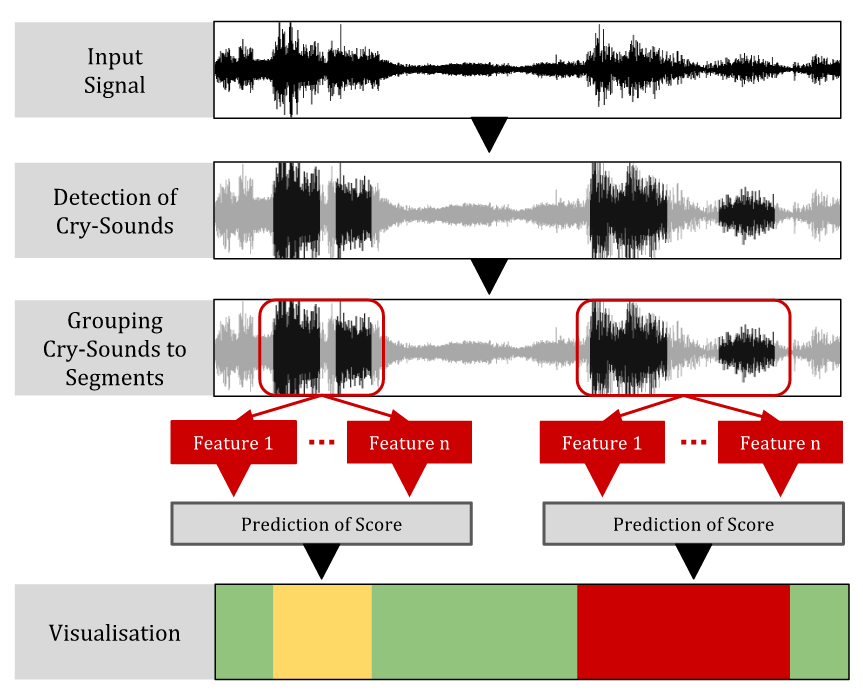
\includegraphics[width=0.9\textwidth]{bilder/konzept03.png}
	\caption{Überblick über die Verarbeitungs-Pipeline}
	\label{img:architecture-overview}
\end{figure}

Der erste Verarbeitungsschritt, die Erkennung der Schreigeräusche, ist notwendig, damit für die Prognose des schmerzbezogenen Scores für das Weinen auch nur solchen Informationen genutzt werden, die tatsächlich vom Weinen eines Baby stammen. Würde man beispielsweise den Score hauptsächlich aus der Tonhöhe des Schreiens ableiten und vorher Störgeräusche wie Hintergrundräusche oder Piepen nicht als solche erkennen, würden die Tonhöhen dieser Geräusche ebenfalls mit in die Berechnungen des Scores einfließen und das Ergebnis verfälschen. Diese Notwendigkeit wurde sowohl von Várallyay \cite{cry_thesis} als auch von Cohen et al. \cite{cohenCry} beschrieben. 

Der zweite Verarbeitungsschritt, die Segmentierung, ist notwendig, da, wie in \autoref{sec:painScores} erläutert, Schmerz-Scores auf Basis der Beobachtung längerer Zeiträume bestimmt werden und in einem kontinuierlichen System sinnvolle Anfangs- und Endzeitpunkte für diese Beobachtungszeiträume gefunden werden müssen. Keine der in \autoref{sec:system_literature} vorgestellten Veröffentlichungen präsentierte ein Methode zur Gruppierung der Schreigeräusche, die für diese Arbeit hätte übernommen werden könnte. Cohen et al. \cite{cohenCry} schlagen eine feste Segmentlänge von 10 Sekunden vor. Es wurde sich gegen diesen Ansatz entschieden, da einige der in \autoref{sec:painScores} beschriebenen Pain-Scales längere Beobachtungszeiträume fordern. In der Promotion von Várallyay \cite{cry_thesis} ist dieser Verarbeitungsschritt nicht notwendig gewesen, da die Analyse nicht kontinuierlich umgesetzt werden musste und die zu analysierenden Segmente manuell geschnitten wurden. Pal et al. \cite{palEmotion} erwähnen keine Gruppierung von Schreigeräuschen. Aus diesem Grund wurde ein simpler Algorithmus zur Segmentierung entwickelt, welcher in \autoref{sec:segmenting} vorgestellt wird.

Die Berechnung von akustischen Eigenschaften des Weinens und der darauf folgenden Prongnose einer Klasse oder eines Wertes ist ein Verarbeitungschritt, der grundlegend in allen in \autoref{sec:system_literature} vorgestellten Veröffentlichungen angewendet wurde. Je nach Ziel der Veröffentlichung werden unterschiedliche Features oder Klassifizierungsmethoden verwendet. Visualisierungsmethoden wurden in keiner Veröffentlichung diskutiert, weshalb ein eigener Ansatz entwickelt wurde.

\section{Schmerzbewertung im multimodalen Verbund}
\label{sec:multimodal_integration}

%Schmissiger Begründung
Aus \autoref{sec:pipeline} geht hervor, dass sich die Visualisierung auf den für den Schmerzindikator \emph{Weinen} vergebenen Score bezieht. Dies würde der Visualisierung eines insgesamten Schmerz-Score entsprechen, insofern anstatt einer multimodalen Schmerz-Scale eine monomodale verwendet wird, welche den Schmerz-Score allein aus dem Weinen ableitet. Ein Beispiel für eine monomodale Schmerz-Scale ist das \glqq Neonatal Facial Coding System\grqq{} (kurz \emph{NFCS}), bei der der Schmerz-Score allein aus der Beobachtung des Schmerzindikators \emph{Gesichtsausdruck} abgeleitet wird.\cite[S. 70]{PainAssessment02} Nach Kenntnis des Autors gibt es keine monomodalen Schmerz-Scale, der sich allein auf das Weinen konzentriert. Es wurde sich dafür entschieden, die Visualisierung allein auf das Scoring des Weinens zu beziehen, da es im Zeitrahmen dieser Arbeit nicht möglich gewesen ist, weitere Methoden für das Scoring andere Schmerzindikatoren zu konzipieren.

Das vorgestellte Konzept lässt sich zur Visualisierung von Schmerz-Scores in einem multimodalen Verbund erweitern. Dazu wird ein Zwischenschritt vor der Visualisierung eingeführt, bei dem die prognostizierten Scores aller weiteren Schmerzindikatoren zur Score des Weinens addiert werden. Dieses Additionsergebnis ist der Schmerz-Score, welcher daraufhin zur Visualisierung genutzt wird. Das in \autoref{sec:visualisation} vorgestellte Visualisierungskonzept lässt sich mit nur leichten Anpassungen übertragen.

\begin{figure}[h]
	\centering
	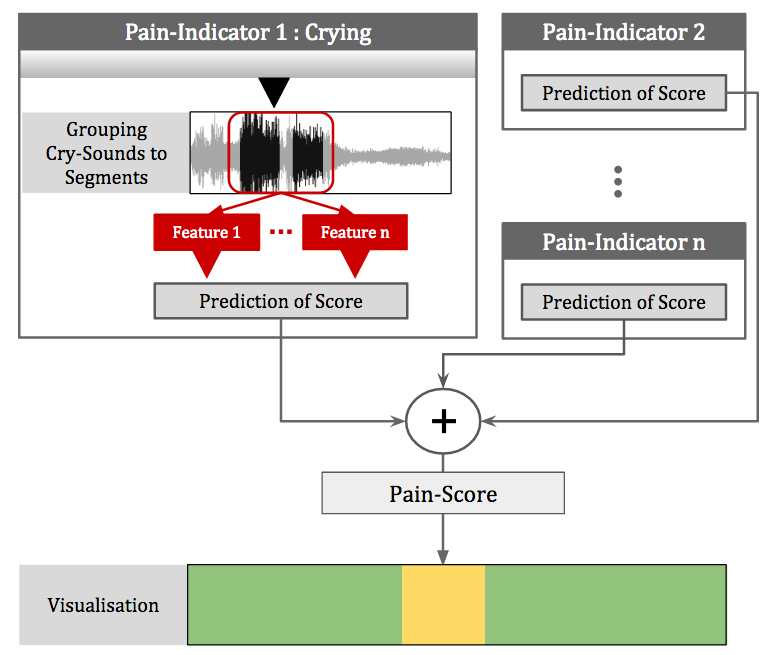
\includegraphics[width=0.7\textwidth]{bilder/multimodal_viz_02.png}
	\caption{Visualisierung im multimodalen Verbund}
	\label{img:multimodal-overview}
\end{figure}